\documentclass{article}
\usepackage[T1]{fontenc}
\usepackage[utf8]{inputenc}
\usepackage[brazil]{babel}

\usepackage{graphicx}
\usepackage{listings}

\lstset{
    basicstyle=\ttfamily
}

\newcommand{\KNNL}{{\lstinline"KNNL"}}
\newcommand{\opencv}{{\lstinline"opencv"}}
\newcommand{\train}{{\lstinline"train"}}

\begin{document}

\title{
    INE5443 --- Reconhecimento de Padrões\\
    Aprendizado de uma paleda de cores por uma rede de Kohonen
}
\author{
    Tiago Royer --- 12100776
}

\maketitle

\section{Problema}

O objetivo era fazer com que uma rede de Kohonen aprendesse uma paleta de cores.

As redes de Kohonen são compostas por uma camada de entrada e uma camada interna;
elas não possuem saída.
Eu coloquei três nodos na camada de entrada;
estes nodos representam as intensidades dos componentes vermelho, verde e azul
na cor que está sendo fornecida na entrada.
A quantidade de nodos na camada interna pode ser definida pelo usuário.

Existe uma conexão entre cada nodo na entrada e cada nodo na camada interna.
Estas conexões foram utilizdas para criar uma visualização da rede.
Um exemplo de execução está disponível na imagem \ref{demo1}.

\begin{figure}[h]
    \centering
    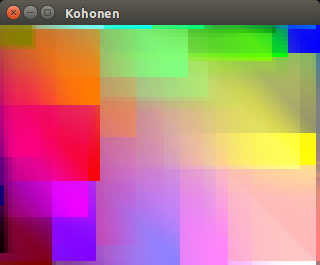
\includegraphics[scale=0.5]{demo1.png}
    \caption{
        Imagem gerada com o comando
        \texttt{./main --size 60 80 --input color\_list.txt --epochs 30 --seed 753}.
    }
    \label{demo1}
\end{figure}

\section{Detalhes da Implementação}

Para implementar as redes neurais, eu utilizei a biblioteca \KNNL.
É uma biblioteca para redes de Kohonen implementada em C++.
Ela é implementada inteiramente em headers
e é distribuída junto do código fonte do programa.

O \opencv foi utilizado para visualização.

\end{document}
